%----------------------------------------------------------------------------
\chapter{Background}
%----------------------------------------------------------------------------
\section{Basics of Unit Testing}

\subsection{A brief introduction to software lifecycle models}
Software development lifecycle models have been used for a long time to support the work of software engineers. These models define the sequence of steps needed to produce a quality software, and they are heavily relied on in large projects. Several models exist, and it is essential to choose the one that is relevant for the project. All of them have testing as a key element though, to verify the correct behaviour of the software product. 

The essence of unit testing can be demonstrated the best in the V-Model (Figure \ref{fig:vmodel}). Its place is next to the detailed design of the software, so that unit tests will verify the requirements on the lowest design level. The model also shows, that unit testing comes immediately after development (writing the source code), and in iterative or other models, testing and development happen in turns or at the same time. \cite{Ruparelia:2010:SDL:1764810.1764814} 

It is also a common practice, to create tests in advance, based on the requirements defined at the start of the project, and then the code under test. This is called test-driven development (TDD), where the goal is to write a program that will make all the tests pass. It often involves software engineers and test engineers as two different teams, so that the software team will have no influence on the tests. TDD will fit in almost any sofware lifecycle model, and it became a popular approach recently. \cite{1510569}


\begin{figure}

\centering
\begin{tikzpicture}[node distance = 1cm, auto]
    % Place nodes
   
    
    \node [block_rounded] (req) {Define\\ requirements};
    \node [block_rounded, below right=1cm and -2.6cm of req] (arch) {System\\ architecture};
    \node [block_rounded, below right=1cm and -2.6cm of arch] (des) {Detailed design};
     \node [block_rounded, below right=1cm and -1cm of des] (dev) {Development};
    \node [block_rounded, above right=1cm and -1cm of dev] (utest) {Build and unit test};
    \node [block_rounded, above right=1cm and -2.6cm of utest] (itest) {System integration and test};
    \node [block_rounded, above right=1cm and -2.6cm of itest] (dep) {Deployment and verification};
    % Draw edges
    \path [line] (req) -- (arch);
    \path [line] (arch) --  (des);
    \path [line] (des) -- (dev);
    \path [line] (dev) -- (utest);
    \path [line] (utest) -- (itest);
    \path [line] (itest) -- (dep);
    \path [double] (des) -- (utest);
    \path [double] (arch) -- (itest);
    \path [double] (req) -- (dep);
    
\end{tikzpicture}

\caption{V-Model: Decomposition and Definition, Integration and Verification} 
\label{fig:vmodel}
\end{figure}
\subsection{Unit testing and testing patterns}
Unit Testing is a main part of the software development workflow, testing of individual hardware or software units or groups of related units \cite{159342}. On the lowest software architecture level, unit tests verify only a single module or package of the code. The tested software runs isolated from other components, external dependencies substituted with custom testing code, so that running a test will not have any effect on the system.Result of a unit test should only depend on the test and the tested software, but no other circumstances. Multiple execution of the same unit test on the same program must produce the exact same output. A test method usually tests a single functionality of the unit, has a set of inputs, and expects a set of outputs or some action to happen.

In a typical tests suite, both positive and negative tests exist. Positive tests exercise the correct behaviour of the software, providing a set of valid inputs, and expecting a defined set of outputs. At the end of the tests, assert methods compare the actual values to the expected ones. Negative tests are for those cases, where the software is expected to fail, an invalid set of inputs for example. Errors like these should be handled in a robust way, like throwing an exception, or returning a value that indicates an error. Most unit test frameworks are able to expect exceptions. \cite{Olan:2003:UTT:948785.948830}

\subsection{Coverage and other metrics}
What makes a good test suite? Code coverage is the most common to be measured, it is the percentage of lines executed in the unit. It gives a good picture about the completeness of the test suite, if all possible functionality is tested. The implementation of this metric is quite simple: a debugger tool marks the lines that have been executed at least once during the execution of the test suite. Speed is also not bad: compared to the bare execution of the tests, the only overhead is the software debugger.

However, code coverage measurement does not reflect to the correlation of the software and the tests. A test quality metric should indicate the ability to find possible errors in the software. Mutation testing is a technique that gives that kind of quality metric. It can be run on a test suite that has all its test cases passing. The first step is to put artificial faults (mutations) in the source code. Then the test suit will be run against the modified program - multiple times, because the faulty programs (mutants) will be exercised one by one. Finally, if the test fails, it was able to "kill" the mutant, and the mutation score will be determined as the ratio of killed mutants to all generated mutants. The mutation can be as simple as flipping a comparison operator, or skipping a jump statement. \cite{aron_mut}\cite{5487526}

Mutation score is a quite accurate metric as test quality, but it is a very resource-demanding process to perform mutation testing: creating mutants is moderately difficult, executing the entire test suite for each mutant however, can be a very long procedure. That is why coverage is preferred to mutation testing most of the time.

\subsection{Test automation}

There have been recent efforts to make unit test creation an automated process, since the simple structure of tests needs often only mechanical coding, instead of a creative process of software design. 

Automatic unit test generation is a major step making software development less resource-consuming and more cost-efficient. Though supervising the process and extending the generated tests are still needed, it may be a lot less time, than writing the whole test manually. Additionally, the generated code will be more likely to be error-free, and will contain test cases the programmer did not think of.

Generating the code of a unit test is rather simple having been given the set of inputs and outputs. After preparing the environment, a function of the tested unit is called with the inputs, and the return value is compared to the expected outputs. The only challenges are to determine, which functions to call (if not specified), and of course what input and output parameters to use. One approach is to create tests randomly, and then keep the useful ones based on the metrics discussed in the previous section.

In certain cases, when a special type of tests are needed, the test generator can be self-made, but most of the cases a more general testing tool with the right parameters is enough. A wide palette of testing tools for most programming languages is available. 

\subsection{IntelliTest}
A popular automatic test generation tool is IntelliTest\footnote{\url{https://visualstudio.microsoft.com/}.}, which is a built-in feature of Microsoft Visual Studio 2015 Enterprise Edition or later. \cite{intellitest_manual}
It supports C\# language projects that target .NET framework. 
\subsection{Java tools}
EvoSuite\footnote{\url{http://www.evosuite.org/}.} is  \cite{aron_autom}
\section{Symbolic execution}

Symbolic execution is a method to define a possible set of inputs for each of the execution paths of the program. It is an extension of normal execution, arithmetic and logic expressions will have to handle symbolic values. Since the program itself will not be modified, symbolic variables will be introduced as inputs. What this means is, that the value of a variable during execution can not only be an integer value, but an expression containing a symbolic variable.
Besides the current values of variables, the execution state contains a path condition. This will be a logical expression showing the current execution path will be followed under what condition. Reaching an If-Else structure the execution can go either way during normal execution, but in this case, both ways must be taken, and the path condition updated with the condition of the branch. If the conditional or its opposite can be proved from the path condition though, only the corresponding branch will be executed. \cite{King:1976:SEP:360248.360252}

When the execution of all branches finish, the result will be a symbolic execution tree, with execution states as nodes, and completed executions as its leafs. The leafs will contain an expression for the path condition, from which the symbolic variables, that are the same as the inputs, will be calculated using a constraint solver.

This way, test inputs for all possible execution paths can be generated, and the test suite will have a 100\% coverage. The method has limitations though. Branching statements will potentially double the number of leafs on the graph, which means in the worst case, that the execution time will grow exponentially with program size. This can restrict the usability of the method on medium or large sized program units. Additionally, the constraint solver might not be compatible, or might be very expensive with all the operations performed in the program (for example nonlinear arithmetic). \cite{z3_tutorial} Operations of a more complex kind, like string manipulation has to be simplified to low-level operations, or treated like a black box. External dependencies have to be mocked or treated like a black box.

\subsection{Java Pathfinder}
\section{About LabVIEW}
LabVIEW is a system engineering software tool, developed by National Instruments, used commonly for rapid development of testing systems, measurement solutions, or other industrial applications. Its features include a graphic programming language, called G, which has advantages over a text-based programming language from a system engineering perspective. The language being graphic comes with a steep learning curve: the drag-and-drop and wiring methods of the software are really intuitive, and the language elements are provided in a toolbox. The program nodes are executed in a data flow, resulting that parallel execution is a natural feature of this language. This is taken advantage of in embedded systems, and it also makes LabVIEW a unique platform for unit testing.
\subsection{The G programming language}
G is a graphical programming language, the source code is called a block diagram. The basic unit of a LabVIEW solution is a Virtual Instrument, or VI for short. VIs correspond to functions in traditional programming languages, they are the containers for G code. Operations are defined as nodes, which have input and output terminals for parameters and return values. Data values are transferred between nodes via wires, which connect an output terminal of a node with one or more input terminals. Controls and indicators are special nodes that connect to the VIs front panel, the user interface of the LabVIEW program. VIs can also be used as subVIs in other VIs, like a function call, in this case controls and indicators become the terminals of the subVI. Case structures and loops are also available, along with lots of other programming features, making G capable of almost anything a traditional programming language can do.

Execution is based on data availability, which means a node will execute, if all its inputs are ready. 
\begin{figure}

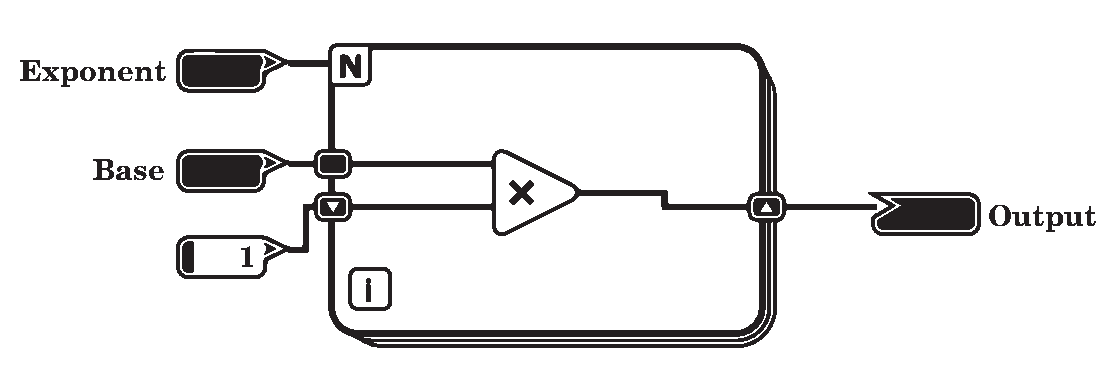
\includegraphics[width=150mm,keepaspectratio]{figures/vi2.pdf}
\caption{Exponent function in G Language} 
\label{fig:gexponent}
\end{figure}

\subsection{Environment and hardware}

The most common LabVIEW solutions are measurement and control applications.
\subsubsection{Measurement tools}
\subsubsection{Real-time hardware}
cRIO

\subsubsection{Dataflow paradigm}
\subsubsection{Built-in nodes}
